\chapter{Interconnessioni elettriche e signal integrity}
Le interconnessioni elettriche svolgono il ruolo funzionale di trasferimento di energia o informazione tra stadi circuitali, identificabili genericamente come un generatore e un carico. Sotto il profilo operativo, si distinguono due categorie strutturali:
\begin{itemize}
    \item \textbf{Reti di potenza} $\rightarrow$ operano a bassa frequenza, compresa nell'intervallo tra pochi Hz e le decine di kHz, gestendo livelli di potenza elevati.
    \begin{figure}[H]
    	\centering
    	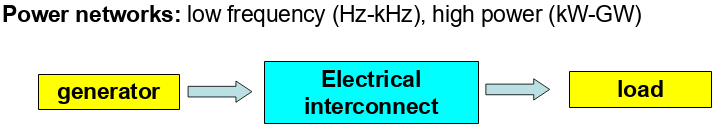
\includegraphics[width=0.55\linewidth]{immagini/signal_integrity}
    \end{figure}
    \item \textbf{Reti di segnale} $\rightarrow$ operano ad alta frequenza, compresa nell'intervallo tra i MHz e i GHz, trasmettendo segnali a bassi livelli di potenza, tipicamente compresi tra milliwatt e watt, tra un trasmettitore o pilota e un dispositivo ricevitore.
    \begin{figure}[H]
    	\centering
    	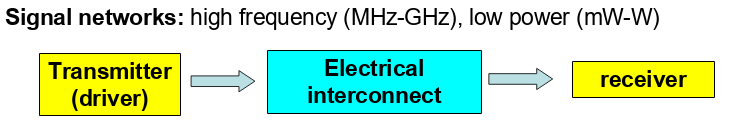
\includegraphics[width=0.55\linewidth]{immagini/signal_integrity1}
    \end{figure}
\end{itemize}

Nelle reti di potenza, lo studio della conformità della forma d'onda della tensione e della corrente ricade nell'ambito della \textbf{power quality}. Tale analisi valuta:
\begin{itemize}
    \item La distorsione armonica generata dalla presenza di carichi non lineari connessi alla rete.
    \item Fenomeni di sovratensione, sottotensione, sovracorrente e sottocorrente rispetto ai valori nominali.
    \item Buchi di tensione transitori sulla linea di alimentazione.
\end{itemize}
I disturbi e le alterazioni indagate dalla power quality non vengono classificati come problemi di compatibilità elettromagnetica.
\begin{figure}[H]
	\centering
	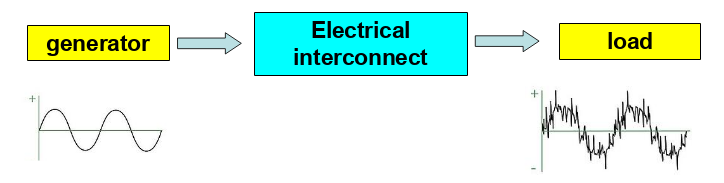
\includegraphics[width=0.6\linewidth]{immagini/signal_integrity2}
\end{figure}

Nelle reti di segnale, l'analisi delle alterazioni subite dalla forma d'onda durante la propagazione lungo l'interconnessione costituisce l'oggetto della \textbf{signal integrity} che verifica:
\begin{itemize}
    \item Qualità del segnale ricevuto $\rightarrow$ fedeltà in ampiezza della forma d'onda ricevuta rispetto alla sorgente, valutando il contenimento di oscillazioni spurie, rumore e degradazione dei livelli logici.
    \item Temporizzazione $\rightarrow$ accuratezza temporale nella propagazione dei fronti di commutazione, rispetto ai margini di sincronizzazione e alle finestre di campionamento del ricevitore.
\end{itemize}

In un \textbf{canale di trasmissione ideale}, l'interconnessione si comporta come un elemento trasparente che preserva integralmente la transizione a gradino dei livelli logici, introducendo solo un ritardo.

Al contrario, in un \textbf{canale di trasmissione reale} l'interconnessione degrada la sequenza di impulsi: i fronti verticali vengono addolciti, i livelli di tensione presentano deformazioni e le ampiezze di picco subiscono variazioni, con conseguente potenziale perdita dell'informazione logica trasmessa.
\begin{figure}[H]
	\centering
	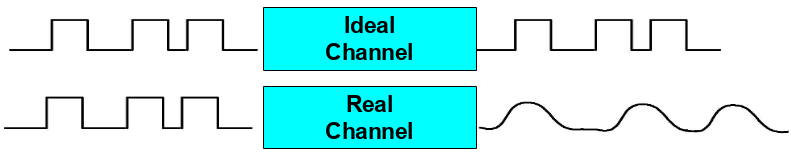
\includegraphics[width=0.7\linewidth]{immagini/signal_integrity3}
\end{figure}

\section{Interconnessioni nei circuiti integrati e ritardo di propagazione}
Nei circuiti ad alta integrazione, l'incrementato della densità circuitale e della miniaturizzazione hanno ridotto progressivamente le dimensioni fisiche dei conduttori. I dati storici dei circuiti integrati commerciali documentano tale andamento:
\begin{center}
\begin{tabular}{|l|c|c|c|c|}
\hline
\hline
\textbf{Parametro del Circuito Integrato} & \textbf{1997} & \textbf{2006} & \textbf{2012} & \textbf{2016} \\
\hline
Area del silicio [$\text{mm}^2$] & $300$ & $520$ & $550$ & $460$ \\
\hline
Numero di transistori [miliardi] & $0.01$ & $0.20$ & $1.4$ & $7.2$ \\
\hline
Larghezza minima delle interconnessioni [$\text{nm}$] & $200$ & $70$ & $35$ & $22$ \\
\hline
Lunghezza complessiva delle interconnessioni [$\text{km}$] & $2.16$ & $5.14$ & $24$ & $100$ \\
\hline
\end{tabular}
\end{center}
L'architettura interna dei microprocessori complessi richiede una rete tridimensionale di conduttori stratificati su molteplici livelli metallici collegati da fori di interconnessione verticali, la cui estensione totale supera i $100\text{ km}$ su un singolo chip.
\begin{figure}[H]
	\centering
	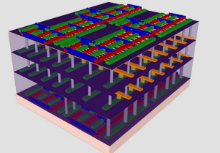
\includegraphics[width=0.3\linewidth]{immagini/signal_integrity4}
\end{figure}

L'impatto primario delle interconnessioni si manifesta nel ritardo complessivo di propagazione del segnale digitale. Nel funzionamento di un circuito logico si distinguono due contributi di ritardo concorrenti:
\begin{itemize}
    \item \textbf{Gate delay} $\rightarrow$ tempo di commutazione del singolo transistore, determinato dalle proprietà intrinseche del dispositivo.
    \item \textbf{Interconnect delay} $\rightarrow$ tempo di transito e propagazione della forma d'onda lungo i conduttori che collegano i dispositivi logici.
\end{itemize}
Con la contrazione del nodo tecnologico, il gate delay diminuisce sensibilmente: i transistori commutano più rapidamente per effetto della riduzione della capacità di gate, dell'abbassamento delle tensioni di alimentazione e dell'accorciamento della lunghezza fisica di canale. All'opposto, il ritardo associato alle interconnessioni non beneficia della scalatura dimensionale e subisce un incremento.
\begin{figure}[H]
	\centering
	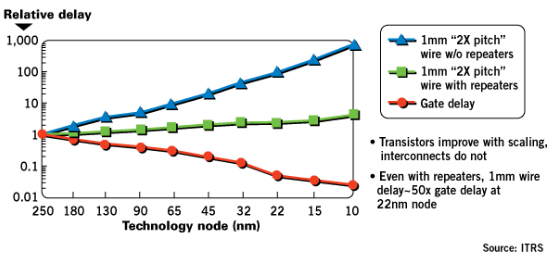
\includegraphics[width=0.6\linewidth]{immagini/signal_integrity5}
\end{figure}

La quantificazione del ritardo introdotto dall'interconnessione si basa sull'approssimazione \textbf{del ritardo di Elmore} per una rete di tipo resistivo-capacitivo: considerando una linea uniforme di lunghezza $L$, avente resistenza per unità di lunghezza $r$ [$\Omega/\text{m}$] e capacità per unità di lunghezza $c$ [$\text{F/m}$], pilotata da una sorgente con resistenza interna $R_s$ e terminata su un carico puramente capacitivo $C_L$, il ritardo di Elmore $t_d$ è espresso dalla relazione:
\[
t_d \simeq R_s (C_L + c L) + r L C_L + \frac{1}{2} r c L^2
\]
L'analisi dei singoli addendi evidenzia il meccanismo fisico di degradazione temporale:
\begin{itemize}
    \item Il termine $R_s (C_L + c L)$ rappresenta la costante di tempo di carica della capacità totale della linea e del carico attraverso la resistenza interna del generatore.
    \item Il termine $r L C_L$ descrive la carica della capacità di carico attraverso la resistenza ohmica totale del conduttore.
    \item Il termine quadratico $\frac{1}{2} r c L^2$ costituisce il ritardo distribuito intrinseco della sola linea di interconnessione.
\end{itemize}

Con il progredire della miniaturizzazione tecnologica:
\begin{itemize}
    \item La resistenza per unità di lunghezza $r$ cresce marcatamente a causa del restringimento della sezione trasversale dei fili metallici.
    \item La capacità per unità di lunghezza $c$ subisce solo una debole diminuzione, restando vincolata dalla vicinanza reciproca delle linee adiacenti.
\end{itemize}
Di conseguenza, il prodotto $r c$ e il contributo $\frac{1}{2} r c L^2$ aumentano in modo considerevole, determinando una crescita esponenziale del ritardo di linea rispetto al tempo di commutazione dei transistori. Nel nodo a $22\text{ nm}$, il ritardo di una traccia metallica di $1\text{ mm}$, pur compensata con stadi di ripetizione, supera di circa $50$ volte il ritardo intrinseco del singolo gate logico.

\section{Strutture guidanti e criteri di modellazione circuitale}
Le interconnessioni operanti ad alta frequenza costituiscono strutture guidanti, nelle quali la direzione di propagazione dell'energia elettromagnetica è vincolata lungo l'asse longitudinale $z$, mentre la propagazione lungo le direzioni trasversali risulta trascurabile. Tipologie diffuse di strutture guidanti comprendono:
\begin{itemize}
    \item Linea bifilare $\rightarrow$ formata da una coppia di conduttori cilindrici paralleli immersi in un mezzo dielettrico omogeneo.
    \item Cavo coassiale $\rightarrow$ costituito da un conduttore cilindrico interno e da uno schermo conduttore tubolare esterno coassiale, separati da un'intercapedine dielettrica uniforme.
    \item Microstriscia $\rightarrow$ realizzata su circuito stampato mediante una pista metallica planare deposta su uno strato di dielettrico supportato da un piano di massa conduttore inferiore.
\end{itemize}
\begin{figure}[H]
	\centering
	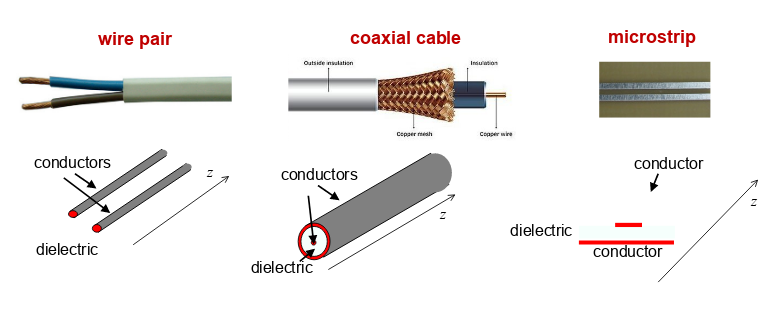
\includegraphics[width=0.8\linewidth]{immagini/signal_integrity6}
\end{figure}

La scelta dell'approccio analitico e computazionale per la simulazione dell'interconnessione richiede una verifica quantitativa basata sul concetto di lunghezza elettrica. La procedura di selezione si articola nelle seguenti fasi:
\begin{enumerate}
    \item Individuazione della massima componente spettrale significativa del segnale $f_{max}$ e della velocità di propagazione nel mezzo $v$.
    \item Calcolo della minima lunghezza d'onda associata:
    \[
    \lambda_{min} = \frac{v}{f_{max}}
    \]
    \item Confronto della lunghezza fisica della linea $\text{len}$ con la frazione $\lambda_{min}/10$.
\end{enumerate}

Le condizioni operative determinano l'impiego di due formulazioni disgiunte:
\begin{itemize}
    \item Condizione a costanti concentrate:
    \[
    \text{len} \le \frac{\lambda_{min}}{10}
    \]
    \item Condizione a parametri distribuiti:
    \[
    \text{len} > \frac{\lambda_{min}}{10}
    \]
\end{itemize}

Nel regime a bassa frequenza, in cui è valida l'approssimazione a parametri concentrati, l'interconnessione viene schematizzata mediante un doppio bipolo equivalente i cui parametri circuitali globali rappresentano differenti meccanismi fisici:
\begin{itemize}
    \item \textbf{$R$} $\rightarrow$ resistenza serie globale, quantificante le perdite per dissipazione Joule lungo i conduttori metallici.
    \item \textbf{$G$} $\rightarrow$ conduttanza parallelo globale, quantificante le perdite per conduzione attraverso il dielettrico interposto.
    \item \textbf{$L$} $\rightarrow$ induttanza magnetica serie globale, associata all'energia immagazzinata nel campo magnetico concatenato con il circuito.
    \item \textbf{$C$} $\rightarrow$ capacità elettrica parallelo globale, associata all'energia immagazzinata nel campo elettrostatico tra i conduttori.
\end{itemize}
Nel modello per la corrente continua intervengono unicamente la resistenza serie $R$ e la conduttanza parallelo $G$. Nel modello per segnali variabili a bassa frequenza intervengono l'induttanza serie $L$ e la capacità parallelo $C$.
\begin{figure}[H]
	\centering
	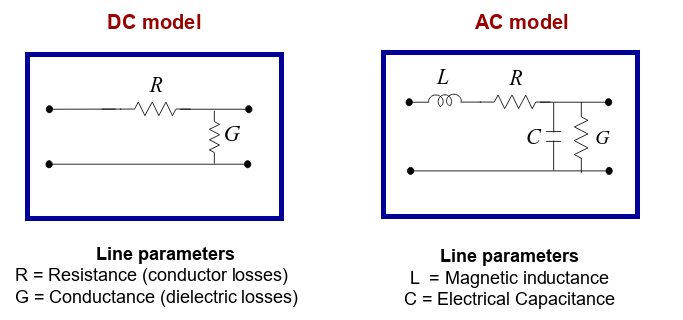
\includegraphics[width=0.65\linewidth]{immagini/signal_integrity7}
\end{figure}

Nel regime ad alta frequenza, in cui la linea risulta elettricamente lunga, l'interconnessione viene discretizzata in una cascata di $N$ celle elementari identiche, ciascuna avente estensione longitudinale $\Delta z$ tale da soddisfare la condizione di brevità elettrica:
\[
\Delta z \le \frac{\lambda_{min}}{10}
\]
Il numero totale di celle elementari necessarie per garantire l'accuratezza della discretizzazione è pari a:
\[
N = \frac{\text{len}}{\Delta z} \ge 10 \frac{\text{len}}{\lambda_{min}}
\]
Ciascuna cella elementare viene descritta dai parametri per unità di lunghezza, definiti dal rapporto tra i parametri globali e la lunghezza totale della traccia:
\[
r = \frac{R}{\text{len}}, \quad l = \frac{L}{\text{len}}, \quad c = \frac{C}{\text{len}}, \quad g = \frac{G}{\text{len}}
\]
\begin{figure}[H]
	\centering
	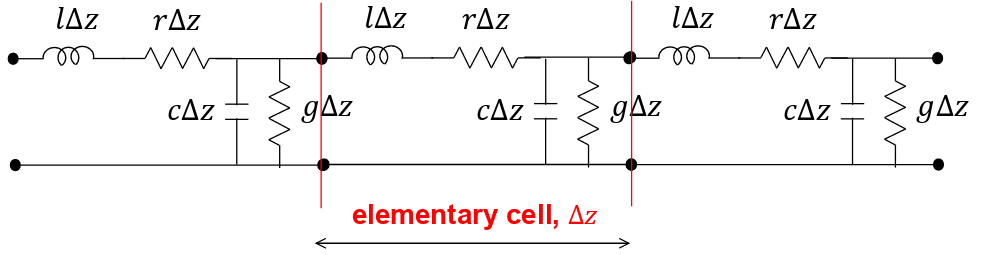
\includegraphics[width=0.7\linewidth]{immagini/signal_integrity8}
\end{figure}
I componenti concentrati della cella elementare assumono i valori $r \Delta z$, $l \Delta z$, $c \Delta z$ e $g \Delta z$.

Applicando i principi di Kirchhoff alle tensioni e alle correnti sulla cella elementare di lunghezza $\Delta z$ compresa tra $z$ e $z + \Delta z$, ed eseguendo il passaggio al limite per $\Delta z \to 0$:
\[
\lim_{\Delta z \to 0} \frac{v(z+\Delta z, t) - v(z,t)}{\Delta z} = - r i(z,t) - l \frac{\partial i(z,t)}{\partial t}
\]
\[
\lim_{\Delta z \to 0} \frac{i(z+\Delta z, t) - i(z,t)}{\Delta z} = - g v(z,t) - c \frac{\partial v(z,t)}{\partial t}
\]
si deducono le equazioni dei telegrafisti nel dominio del tempo, valide nell'intervallo spaziale tra $z = 0$ e $z = \text{len}$:
\[
-\frac{\partial v(z,t)}{\partial z} = r i(z,t) + l \frac{\partial i(z,t)}{\partial t}
\]
\[
-\frac{\partial i(z,t)}{\partial z} = g v(z,t) + c \frac{\partial v(z,t)}{\partial t}
\]

Sotto il profilo dell'interpretazione elettromagnetica, la propagazione lungo la struttura guidante si scompone in modi spaziali:
\begin{itemize}
    \item \textbf{Modo TEM} (trasverso elettro-magnetico) $\rightarrow$ costituisce il modo fondamentale privo di frequenza di taglio ($f_c = 0$), in grado di propagarsi a qualunque frequenza. In tale configurazione sia il campo elettrico che il campo magnetico giacciono rigorosamente nel piano trasversale ortogonale alla direzione di propagazione ($E_z = 0$, $H_z = 0$).
    \item Modi di ordine superiore $\rightarrow$ comprendono i modi trasversi elettrici \textbf{TE} ($E_z = 0$, $H_z \ne 0$) e i modi trasversi magnetici \textbf{TM} ($H_z = 0$, $E_z \ne 0$), ciascuno caratterizzato da una specifica frequenza di taglio non nulla.
\end{itemize}

I criteri di validità per la formulazione matematica del problema sono governati dalla frequenza di eccitazione:
\begin{itemize}
    \item Se la frequenza del segnale si mantiene al di sotto della frequenza di taglio del primo modo di ordine superiore, si propaga unicamente il modo fondamentale trasverso elettro-magnetico. Il comportamento dell'interconnessione è descritto integralmente dal modello a linea di trasmissione, le cui incognite sono grandezze circuitali scalari dipendenti da spazio e tempo, ossia la tensione $v(z,t)$ e la corrente $i(z,t)$.
    \item Se la frequenza supera la soglia di taglio dei modi superiori, insorgono fenomeni di propagazione tridimensionale. Il modello a linea di trasmissione decade ed è obbligatorio risolvere le equazioni elettromagnetiche a onda intera full-wave, le cui incognite sono i campi vettoriali nello spazio tridimensionale $\mathbf{E}(\mathbf{r},t)$ e $\mathbf{B}(\mathbf{r},t)$.
\end{itemize}

La differenza concettuale tra le due formulazioni circuitali si riflette sulla distribuzione spaziale delle grandezze:
\begin{itemize}
    \item Nel modello a costanti concentrate l'interconnessione non manifesta effetti di propagazione spaziale; tensione e corrente dipendono esclusivamente dal tempo, risultando uniformi lungo l'intera coordinata $z$:
    \[
    v(t), \quad i(t)
    \]
    \item Nel modello a parametri distribuiti la tensione e la corrente manifestano un'esplicita dipendenza congiunta da spazio e tempo:
    \[
    v(z,t), \quad i(z,t)
    \]
    lungo la linea si stabilisce un profilo stazionario o viaggiante con ondeggiamenti spaziali di ampiezza $|V(z)|$ tra la coordinata di ingresso $z = 0$ e la coordinata di carico $z = \text{len}$.
\end{itemize}
\begin{figure}[H]
	\centering
	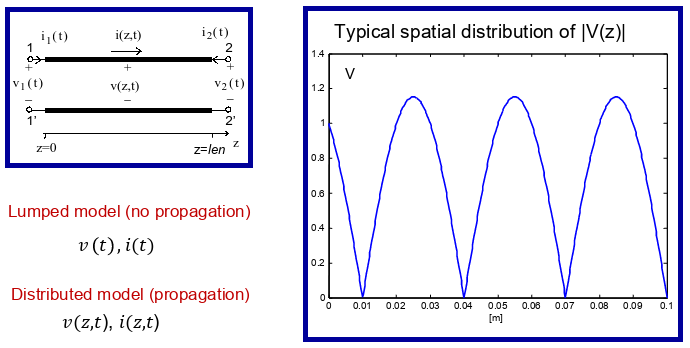
\includegraphics[width=0.8\linewidth]{immagini/signal_integrity9}
\end{figure}

\subsection{Parametri per unità di lunghezza}
I parametri distribuiti di induttanza $l$ e capacità $c$ per unità di lunghezza dipendono unicamente dalla geometria della sezione trasversale e dalle proprietà costitutive dei materiali dielettrici e magnetici:
\begin{itemize}
    \item Cavo coassiale, con raggio del conduttore centrale pari ad $a$, raggio interno dello schermo esterno pari a $b$, permeabilità magnetica $\mu$ e permittività dielettrica $\varepsilon$:
    \begin{figure}[H]
    	\centering
    	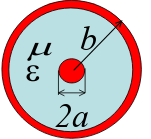
\includegraphics[width=0.15\linewidth]{immagini/signal_integrity10}
    \end{figure}
    \[
    l = \frac{\mu}{2\pi} \ln\left(\frac{b}{a}\right)
    \]
    \[
    c = \frac{2\pi\varepsilon}{\ln\left(\frac{b}{a}\right)}
    \]
    \item Linea bifilare, costituita da due conduttori cilindrici paralleli di raggio $a$ (diametro $2a$) posti a interasse reciproco $d$:
    \begin{figure}[H]
    	\centering
    	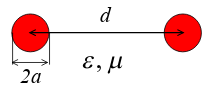
\includegraphics[width=0.25\linewidth]{immagini/signal_integrity11}
    \end{figure}
    \[
    L' = \frac{\mu}{\pi} \ln\left(\frac{d-a}{a}\right)
    \]
    \[
    C' = \frac{\pi\varepsilon}{\ln\left(\frac{d-a}{a}\right)}
    \]
\end{itemize}

La quantificazione della resistenza per unità di lunghezza $r$ richiede la distinzione del regime di frequenza in relazione all'effetto pelle. Lo spessore di penetrazione $\delta$ del conduttore metallico avente conducibilità elettrica $\sigma$ e permeabilità $\mu$ alla frequenza $f$ è definito da:
\[
\delta = \sqrt{\frac{1}{\pi \sigma \mu f}}
\]

In regime di bassa frequenza, in cui lo spessore di penetrazione $\delta$ risulta maggiore delle dimensioni trasversali del conduttore, l'effetto pelle è assente e la densità di corrente è uniformemente distribuita su tutta l'area metallica $S$. La resistenza per unità di lunghezza coincide con il valore in corrente continua:
\begin{itemize}
    \item Per conduttore a sezione rettangolare di larghezza $W$ e spessore $H$, con area $S = W H$:
    \[
    r_{DC} = \frac{1}{\sigma S} = \frac{1}{\sigma W H}
    \]
    \item Per conduttore a sezione circolare di raggio $r_W$, con area $S = \pi r_W^2$:
    \[
    r_{DC} = \frac{1}{\sigma S} = \frac{1}{\sigma \pi r_W^2}
    \]
\end{itemize}

In regime di alta frequenza, in cui lo spessore di penetrazione $\delta$ diventa molto inferiore alle dimensioni trasversali, la corrente si addensa in un sottile strato perimetrale di spessore $\delta$. La sezione geometrica efficace di conduzione $S_{eff}$ coincide approssimativamente con il prodotto tra il perimetro del conduttore e lo spessore $\delta$. La resistenza per unità di lunghezza assume il valore:
\begin{itemize}
    \item Per conduttore rettangolare con perimetro $2(W + H)$:
    \[
    r_{HF} = \frac{1}{\sigma S_{eff}} = \frac{1}{2\sigma (W + H)} \sqrt{\frac{\mu}{\pi \sigma}} \sqrt{f}
    \]
    \item Per conduttore circolare di raggio $r_W$:
    \[
    r_{HF} = \frac{1}{\sigma S_{eff}} = \frac{1}{2 r_W} \sqrt{\frac{\mu}{\pi \sigma}} \sqrt{f}
    \]
\end{itemize}
Ad alta frequenza, la resistenza ohmica della linea aumenta proporzionalmente alla radice quadrata della frequenza $\sqrt{f}$.
\begin{figure}[H]
	\centering
	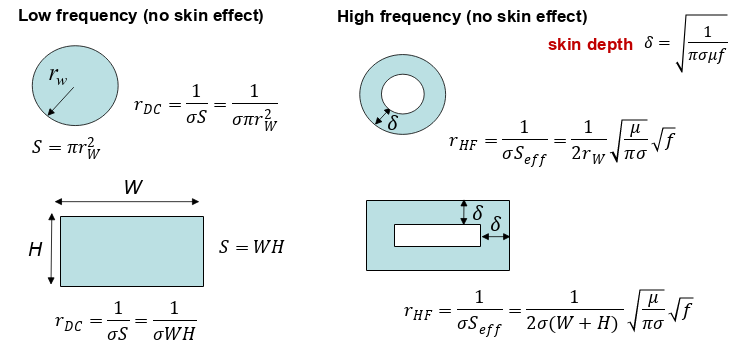
\includegraphics[width=0.8\linewidth]{immagini/signal_integrity12}
\end{figure}

\subsection{Modello della linea di trasmissione ideale}
Nel caso ideale di interconnessione priva di perdite, i parametri dissipativi sono nulli ($r = 0$, $g = 0$). Le equazioni dei telegrafisti nel dominio del tempo si riducono a:
\[
-\frac{\partial v(z,t)}{\partial z} = l \frac{\partial i(z,t)}{\partial t}
\]
\[
-\frac{\partial i(z,t)}{\partial z} = c \frac{\partial v(z,t)}{\partial t}
\]
Derivando la prima equazione rispetto a $z$ e sostituendo la seconda derivata temporale della corrente, si ottiene l'equazione delle onde unidimensionale di D'Alembert per la tensione:
\[
\frac{\partial^2 v(z,t)}{\partial z^2} - l c \frac{\partial^2 v(z,t)}{\partial t^2} = 0
\]
I parametri caratteristici della propagazione d'onda risultano:
\begin{itemize}
    \item \textbf{$v$} $\rightarrow$ velocità di propagazione dell'onda elettromagnetica lungo la linea:
    \[
    v = \frac{1}{\sqrt{l c}} = v_{em}
    \]
    \item \textbf{$Z_0$} $\rightarrow$ impedenza caratteristica della linea:
    \[
    Z_0 = \sqrt{\frac{l}{c}}
    \]
    \item \textbf{$T$} $\rightarrow$ tempo di transito necessario all'onda per percorrere l'intera tratta $\text{len}$:
    \[
    T = \frac{\text{len}}{v} = \text{len} \sqrt{l c}
    \]
\end{itemize}

La soluzione generale dell'equazione delle onde si esprime come sovrapposizione lineare di un'onda progressiva propagante in direzione $+z$ e di un'onda regressiva propagante in direzione $-z$:
\[
V(z,t) = V^+\left(t - \frac{z}{v}\right) + V^-\left(t + \frac{z}{v}\right)
\]
La corrispondente distribuzione spaziale e temporale della corrente è legata alla tensione tramite l'impedenza caratteristica:
\[
I(z,t) = \frac{1}{Z_0} V^+\left(t - \frac{z}{v}\right) - \frac{1}{Z_0} V^-\left(t + \frac{z}{v}\right)
\]

Si consideri un circuito formato da un generatore reale con tensione impressa $v_s(t)$ e resistenza interna $R_s$ connesso all'ingresso $z = 0$, e da una resistenza di carico $R_L$ posta alla terminazione $z = \text{len}$. Il comportamento dinamico della tensione ricevuta $v_L(t)$ ai capi del carico dipende dal rapporto tra $R_L$ e $Z_0$:
\begin{itemize}
    \item Condizione di adattamento:
    \[
    R_L = Z_0
    \]
    Il coefficiente di riflessione al carico è nullo e non si genera alcuna onda regressiva ($V^- = 0$). Il segnale ricevuto sul carico riproduce la forma d'onda del generatore traslata nel tempo del ritardo di propagazione $T$, senza alcuna alterazione di forma o oscillazione spuria.
    \begin{figure}[H]
    	\centering
    	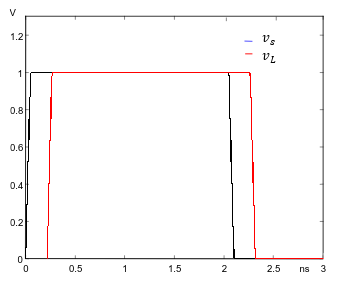
\includegraphics[width=0.35\linewidth]{immagini/signal_integrity13}
    \end{figure}
    
    \item Condizione ad alta impedenza:
    \[
    R_L > Z_0
    \]
    Il disadattamento genera un coefficiente di riflessione positivo al carico. L'onda riflessa si somma in concordanza di fase all'onda incidente, producendo sovraelongazioni rispetto al valore di regime. La tensione sul carico esibisce un andamento oscillatorio a gradini smorzati, che supera la soglia di ampiezza logica prima di stabilizzarsi.
    \begin{figure}[H]
    	\centering
    	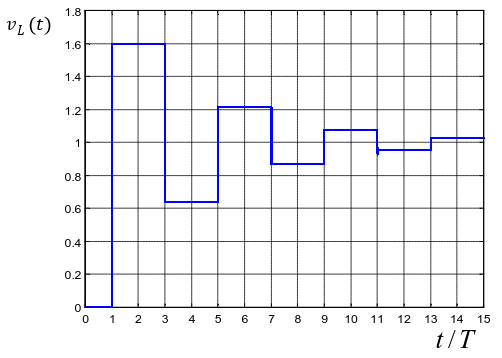
\includegraphics[width=0.4\linewidth]{immagini/signal_integrity14}
    \end{figure}
    	
    \item Condizione a bassa impedenza:
    \[
    R_L < Z_0
    \]
    Il disadattamento genera un coefficiente di riflessione negativo al carico. L'onda riflessa sottrae ampiezza all'onda incidente, determinando sottoelongazioni. La tensione sul carico raggiunge il valore di regime attraverso una salita a gradini ritardata, con una transizione iniziale di ampiezza insufficiente a superare la soglia di commutazione.
    \begin{figure}[H]
    	\centering
    	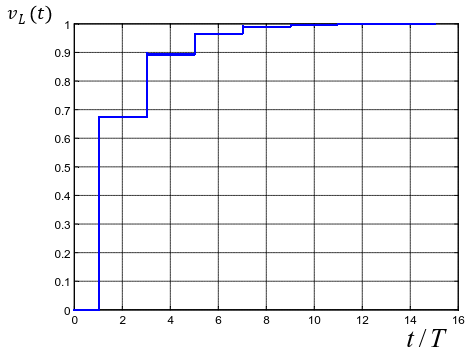
\includegraphics[width=0.4\linewidth]{immagini/signal_integrity15}
    \end{figure}
    
\end{itemize}

Nelle linee reali con perdite, la propagazione è descritta dal \textbf{modello quasi-TEM}:
\begin{itemize}
    \item Con perdite indipendenti dalla frequenza, quantificate dalla resistenza per unità di lunghezza costante $r$ e dalla conduttanza $g$.
    \item Con perdite dipendenti dalla frequenza, descritte dall'impedenza per unità di lunghezza $Z(\omega)$ e dall'ammettenza per unità di lunghezza $Y(\omega)$.
\end{itemize}
Le equazioni dei telegrafisti nel dominio della frequenza assumono la forma:
\[
-\frac{d V(z,\omega)}{dz} = Z(\omega) I(z,\omega)
\]
\[
-\frac{d I(z,\omega)}{dz} = Y(\omega) V(z,\omega)
\]

La \textbf{presenza delle perdite} introduce degradazioni aggiuntive sulla forma d'onda ricevuta $v_L(t)$ visibili dal seguente grafico:
\begin{figure}[H]
	\centering
	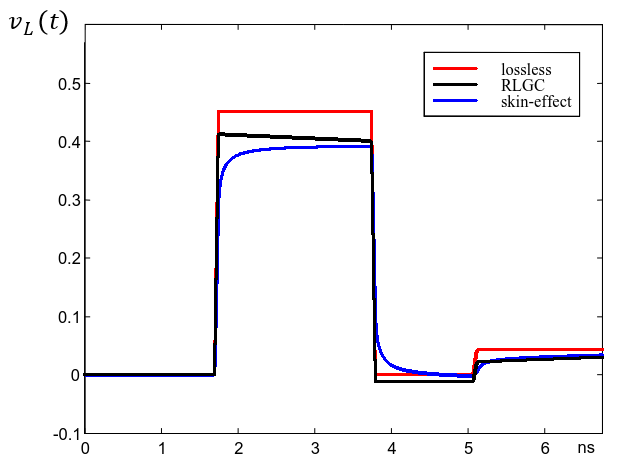
\includegraphics[width=0.4\linewidth]{immagini/signal_integrity16}
\end{figure}
\begin{itemize}
    \item Nel caso ideale privo di perdite, l'impulso perviene sul carico perfettamente integro, traslato unicamente del tempo di transito $T$.
    \item Nel modello con parametri dissipativi costanti, l'impulso subisce attenuazione di ampiezza e una lieve inclinazione del tetto orizzontale, ma preserva la pendenza dei fronti di salita.
    \item Nel modello con perdite dipendenti dalla frequenza governate dall'effetto pelle, le armoniche spettrali ad alta frequenza vengono fortemente attenuate e si innesca la dispersione di fase. La forma d'onda ricevuta manifesta una netta distorsione caratterizzata dall'arrotondamento del fronte di commutazione e dalla formazione di una coda lenta a lungo tempo di assestamento.
\end{itemize}

\section{Modellazione nel dominio del tempo e approccio SPICE}
Per consentire la simulazione transitoria delle linee di trasmissione in circuiti non lineari complessi, si adotta una rappresentazione alternativa a doppio bipolo nel dominio del tempo, nota come modello di Branin o formulazione basata sulle caratteristiche.
\begin{figure}[H]
	\centering
	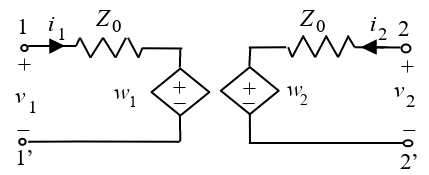
\includegraphics[width=0.4\linewidth]{immagini/signal_integrity17}
\end{figure}
Considerando una linea ideale priva di perdite avente impedenza caratteristica $Z_0$ e tempo di transito $T$, le relazioni costitutive alle due porte terminali $1$ ($z = 0$) e $2$ ($z = \text{len}$) sono espresse dal sistema:
\[
\begin{cases}
v_1(t) - Z_0 i_1(t) = w_1(t) \\
v_2(t) - Z_0 i_2(t) = w_2(t)
\end{cases}
\]
dove le sorgenti di tensione controllate $w_1(t)$ e $w_2(t)$ sono definite ritardando le grandezze dell'estremo opposto:
\[
\begin{cases}
w_1(t) = v_2(t - T) + Z_0 i_2(t - T) \\
w_2(t) = v_1(t - T) + Z_0 i_1(t - T)
\end{cases}
\]
con condizioni iniziali nulle:
\[
w_1(t) = 0, \quad w_2(t) = 0 \quad \text{per } t < T
\]
Il significato fisico delle variabili d'onda corrisponde alla propagazione dell'informazione:
\begin{itemize}
    \item \textbf{$w_1(t)$} $\rightarrow$ rappresenta alla porta $1$ all'istante attuale $t$ gli eventi di tensione e corrente verificatisi alla porta $2$ all'istante antecedente $t - T$.
    \item \textbf{$w_2(t)$} $\rightarrow$ rappresenta alla porta $2$ all'istante attuale $t$ gli eventi di tensione e corrente verificatisi alla porta $1$ all'istante antecedente $t - T$.
\end{itemize}

Nell'algoritmo iterativo implementato nel simulatore SPICE, l'asse temporale viene discretizzato negli istanti sequenziali:
\[
t_n = n \Delta t \quad \text{con } n = 0, 1, 2, \dots
\]
All'istante generico $t_n$:
\begin{itemize}
    \item Le grandezze ritardate $v_1(t_n - T)$, $i_1(t_n - T)$, $v_2(t_n - T)$ e $i_2(t_n - T)$ appartengono a passi di simulazione precedenti già calcolati e registrati in memoria, poiché $t_n - T < t_n$.
    \item Di conseguenza, i valori istantanei delle sorgenti di tensione:
    \[
    W_1(t_n) = v_2(t_n - T) + Z_0 i_2(t_n - T) \quad \text{per } t_n \ge T
    \]
    \[
    W_2(t_n) = v_1(t_n - T) + Z_0 i_1(t_n - T) \quad \text{per } t_n \ge T
    \]
    rappresentano termini noti e costanti all'istante corrente.
\end{itemize}
Il modello a linea di trasmissione si disaccoppia istante per istante in una coppia di circuiti equivalenti di Thévenin indipendenti alle due porte:
\begin{figure}[H]
	\centering
	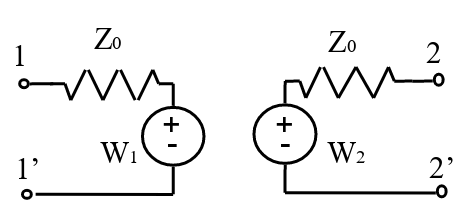
\includegraphics[width=0.4\linewidth]{immagini/signal_integrity18}
\end{figure}
La porta $1$ vede un generatore di tensione ideale $W_1$ con resistenza serie $Z_0$, e la porta $2$ vede un generatore $W_2$ con resistenza serie $Z_0$. Il simulatore risolve le due terminazioni separatamente senza dover invertire matrici globali accoppiate nel dominio del tempo.

Nel caso specifico in cui la linea risulti chiusa su un carico perfettamente adattato alla porta $2$ ($R_L = Z_0$):
\begin{figure}[H]
	\centering
	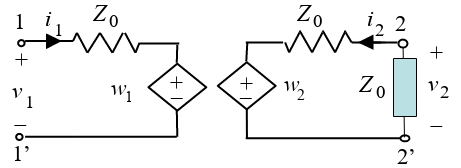
\includegraphics[width=0.5\linewidth]{immagini/signal_integrity19}
\end{figure}
\[
v_2(t) = - Z_0 i_2(t)
\]
Sostituendo tale relazione nell'espressione della sorgente d'onda retrograda:
\[
w_1(t) = v_2(t - T) + Z_0 i_2(t - T) = - Z_0 i_2(t - T) + Z_0 i_2(t - T) = 0
\]
La sorgente $w_1(t)$ si annulla identicamente per ogni istante di tempo. Il circuito equivalente alla porta di ingresso si semplifica nella sola resistenza pura $Z_0$:
\[
v_1(t) = Z_0 i_1(t)
\]
\begin{figure}[H]
	\centering
	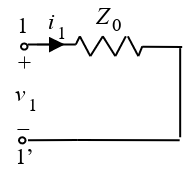
\includegraphics[width=0.2\linewidth]{immagini/signal_integrity20}
\end{figure}
Alla porta di uscita, la tensione coincide direttamente con la tensione di ingresso ritardata:
\[
v_2(t) = v_1(t - T)
\]

\newpage
\section{Esempio di problema di signal integrity}
Per segnali logici digitali ad alta velocità, la determinazione della tipologia di modello circuitale non può fare riferimento a una singola frequenza sinusoidale, ma deve basarsi sulla dinamica di commutazione degli impulsi. Il criterio alternativo per segnali digitali definisce la banda a $3\text{ dB}$ dell'impulso a partire dal tempo di salita $t_r$:
\[
f_{3\text{dB}} \approx \frac{0.35}{t_r}
\]
Assumendo per stima conservativa la frequenza massima come inversamente proporzionale al tempo di salita, la minima lunghezza d'onda associata risulta legata alla transizione temporale:
\[
\lambda_{min} = \frac{v}{f_{3\text{dB}}} \approx v \cdot t_r
\]
Esprimendo la lunghezza della traccia attraverso il tempo di transito $T = \text{len}/v$, il rapporto geometrico fondamentale diventa:
\[
\frac{\text{len}}{\lambda_{min}} \approx \frac{T}{t_r}
\]
Il numero minimo di celle elementari necessarie per la modellazione a cascata di una linea digitale soddisfa la disuguaglianza:
\[
N \ge 10 \frac{\text{len}}{\lambda_{min}} \approx 10 \frac{T}{t_r}
\]

Come esempio applicativo dei criteri generali e alternativi, si consideri una traccia digitale avente:
\begin{itemize}
    \item Lunghezza fisica $\text{len} = 10\text{ cm}$.
    \item Tempo di salita del segnale $t_r = 0.2\text{ ns}$.
    \item Capacità per unità di lunghezza $c = 1\text{ pF/cm}$.
    \item Induttanza per unità di lunghezza $l = 5\text{ nH/cm}$.
\end{itemize}
La velocità di propagazione associata è:
\[
v = \frac{1}{\sqrt{l c}} = \frac{1}{\sqrt{500 \cdot 10^{-9} \cdot 100 \cdot 10^{-12}}} \approx 1.414 \cdot 10^8\text{ m/s} = 14.14\text{ cm/ns}
\]
Il tempo di transito risulta:
\[
T = \frac{\text{len}}{v} = \frac{10\text{ cm}}{14.14\text{ cm/ns}} \approx 0.707\text{ ns}
\]
Il rapporto tra tempo di transito e tempo di salita vale $T/t_r \approx 3.535$, imponendo un numero di celle discretizzate pari a:
\[
N \ge 10 \frac{T}{t_r} \approx 35
\]

Un problema tipico di signal integrity è costituito dalla trasmissione del segnale di clock attraverso le piste di un package per circuiti integrati:
\begin{figure}[H]
	\centering
	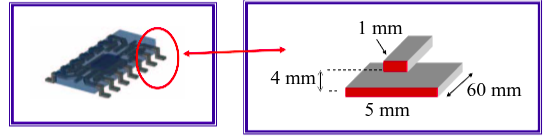
\includegraphics[width=0.5\linewidth]{immagini/signal_integrity22}
\end{figure}
Si consideri una traccia di package con estensione longitudinale pari a $60\text{ mm}$, interfacciata a strutture con dimensioni trasversali caratteristiche comprese tra $1\text{ mm}$ e $5\text{ mm}$. I parametri distribuiti della linea sono:
\begin{itemize}
    \item \textbf{$\text{len} = 60\text{ mm}$} $\rightarrow$ lunghezza totale dell'interconnessione su package.
    \item \textbf{$l = 0.324\ \mu\text{H/m}$} $\rightarrow$ induttanza per unità di lunghezza.
    \item \textbf{$c = 34.37\text{ pF/m}$} $\rightarrow$ capacità per unità di lunghezza.
    \item \textbf{$Z_0 = 97.02\ \Omega$} $\rightarrow$ impedenza caratteristica della traccia.
    \item \textbf{$T = 0.2\text{ ns}$} $\rightarrow$ tempo di transito lungo l'interconnessione.
\end{itemize}

\begin{figure}[H]
	\centering
	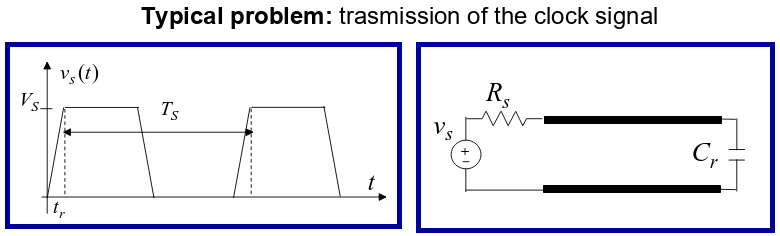
\includegraphics[width=0.7\linewidth]{immagini/signal_integrity21}
\end{figure}
Il generatore di clock fornisce una tensione periodica con ampiezza $V_s = 1\text{ V}$, resistenza interna nulla ($R_s = 0\ \Omega$), periodo $T_s$ e tempo di salita $t_r$. Il ricevitore presenta un carico capacitivo $C_r$. La soglia logica di commutazione del ricevitore è fissata a $V_{th} = 0.5\text{ V}$.

L'analisi comparativa mette a confronto la risposta transitoria ottenuta con due modelli circuitali alternativi:
\begin{itemize}
    \item Modello a parametri distribuiti $\rightarrow$ implementato come linea di trasmissione ideale governata dalle equazioni differenziali dei telegrafisti.
    \item Modello a costanti concentrate $\rightarrow$ implementato mediante una singola cella equivalente con induttanza concentrata $L = l \times \text{len} = 19.44\text{ nH}$ e capacità concentrata $C = c \times \text{len} = 2.06\text{ pF}$.
\end{itemize}
\begin{figure}[H]
	\centering
	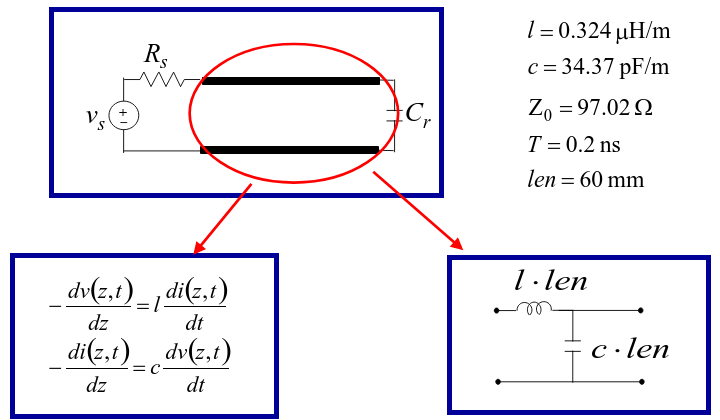
\includegraphics[width=0.6\linewidth]{immagini/signal_integrity23}
\end{figure}

\newpage
Il comportamento dei due modelli viene valutato al variare della frequenza del clock, riducendo progressivamente i parametri temporali $t_r$ e $T_s$:
\begin{enumerate}
    \item Regime a bassa frequenza, con $V_s = 1\text{ V}$, $R_s = 0\ \Omega$, $C_r = 1\text{ nF}$, $t_r = 1\ \mu\text{s}$ e periodo $T_s = 9\ \mu\text{s}$:
    Il tempo di salita $t_r = 1\ \mu\text{s}$ supera di ordini di grandezza il tempo di transito della linea $T = 0.2\text{ ns}$ ($t_r \gg T$). Le risposte nel dominio del tempo fornite dal modello distribuito e dal modello concentrato risultano indistinguibili, sovrapponendosi perfettamente. L'istante di attraversamento della soglia $V_{th} = 0.5\text{ V}$ coincide tra i due modelli, l'errore di sincronizzazione è nullo e il margine temporale in cui il segnale staziona al livello logico alto è massimo. Il modello a parametri concentrati è pienamente accurato.
    \begin{figure}[H]
    	\centering
    	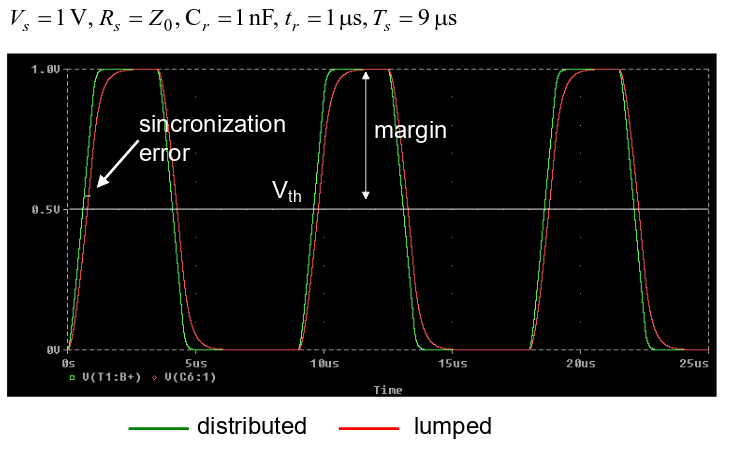
\includegraphics[width=0.7\linewidth]{immagini/signal_integrity24}
    \end{figure}

    \item Regime a media frequenza, con $V_s = 1\text{ V}$, $R_s = 0\ \Omega$, $C_r = 0.1\text{ nF}$, $t_r = 0.1\ \mu\text{s}$ ($100\text{ ns}$) e periodo $T_s = 0.9\ \mu\text{s}$:
    La risposta del modello a costanti concentrate si discosta nettamente dalla risposta distribuita: mentre il modello distribuito riproduce un fronte ripido che raggiunge stabilmente $1\text{ V}$, il modello concentrato mostra una transizione arrotondata con picco massimo ridotto a circa $0.8\text{ V}$. L'attraversamento della soglia $V_{th} = 0.5\text{ V}$ avviene con un ritardo consistente, generando un errore di sincronizzazione significativo e una contrazione del margine temporale utile.
    \begin{figure}[H]
    	\centering
    	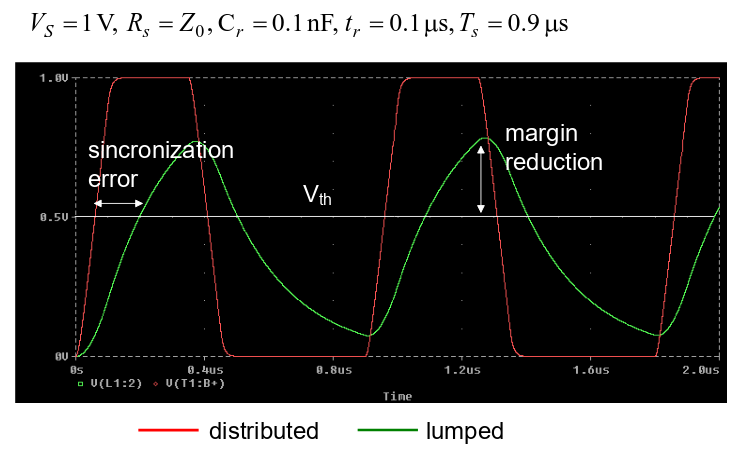
\includegraphics[width=0.7\linewidth]{immagini/signal_integrity25}
    \end{figure}

	\newpage
    \item Regime ad alta frequenza, con $V_s = 1\text{ V}$, $R_s = 0\ \Omega$, $C_r = 0.01\text{ nF}$ ($10\text{ pF}$), $t_r = 10\text{ ns}$ e periodo $T_s = 90\text{ ns}$:
    Il modello a parametri distribuiti riproduce commutazioni nette e stabili tra $0\text{ V}$ e $1\text{ V}$. Al contrario, il modello a costanti concentrate fallisce in modo catastrofico: la forma d'onda concentrata degrada in una perturbazione di bassissima ampiezza che oscilla al di sotto di $0.3\text{ V}$, senza mai intersecare la soglia logica $V_{th} = 0.5\text{ V}$. L'impiego del modello concentrato porterebbe a concludere erroneamente che il circuito logico sia non funzionante e bloccato allo stato zero, evidenziando la totale inadeguatezza dei modelli a celle singole per la predizione della signal integrity ad alta velocità.
    \begin{figure}[H]
    	\centering
    	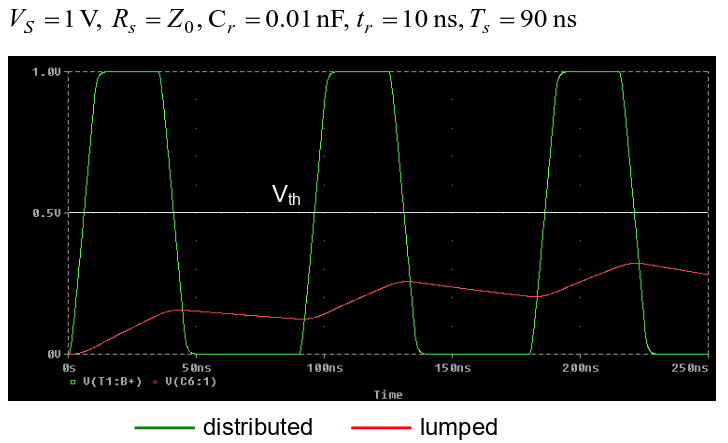
\includegraphics[width=0.7\linewidth]{immagini/signal_integrity26}
    \end{figure}
	

    \item Regime a frequenza ultra-elevata, con $V_s = 1\text{ V}$, $R_s = 0\ \Omega$, $C_r = 0.1\text{ pF}$, $t_r = 0.09\text{ ns}$ ($90\text{ ps}$) e periodo $T_s = 0.3\text{ ns}$ ($300\text{ ps}$):
    In queste condizioni la frequenza fondamentale del clock supera i gigahertz e la lunghezza d'onda minima $\lambda$ diventa comparabile con le dimensioni geometriche trasversali dell'interconnessione e del package ($\lambda \approx \text{dimensione trasversale}$). Si manifesta il limite di validità della stessa teoria delle linee di trasmissione: il modo trasverso elettro-magnetico non è più l'unico modo propagante, insorgono modi di ordine superiore e risonanze di cavità tridimensionali. Il modello a parametri distribuiti diverge dalla risposta fisica reale, rendendo indispensabile l'analisi elettromagnetica full-wave tridimensionale, che evidenzia forti oscillazioni parassite, accoppiamenti e sovraelongazioni negative.
    \begin{figure}[H]
    	\centering
    	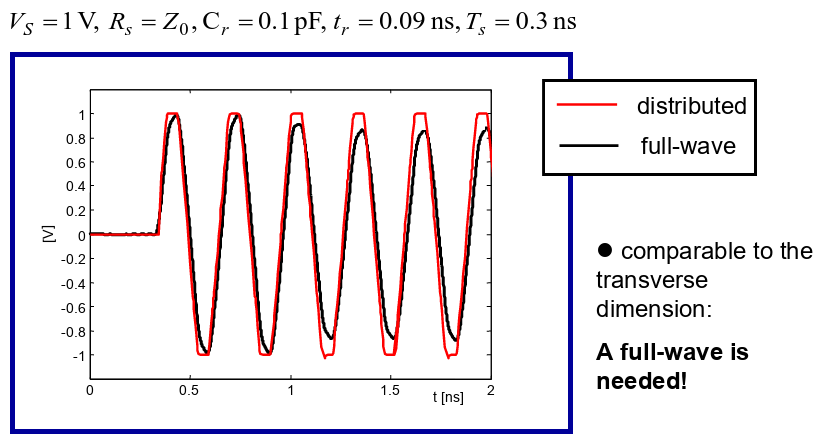
\includegraphics[width=0.7\linewidth]{immagini/signal_integrity27}
    \end{figure}
    
\end{enumerate}

